% Provenance (never printed): see sources/outline_sources.md (Year 1: compaction and
% cementation; basin types; subsidence, accommodation and sea-level change). Exercise and
% problem values in the Book 3 scratch calculator calc/ch23.py; figure data from
% figdata/bachelor-1/compaction.py and sea_level.py.
% Porosity and permeability are Book 1's (g6); diagenesis was met in Book 2 (g12) and is
% re-founded here; sedimentary basin was met in Book 2 (g11) and is re-founded here;
% isostasy and the equal-mass proposition are ch. 11's; passive margins and rifts ch. 13's;
% effective stress ch. 16's; the Last Glacial Maximum and glacial cycles Book 2's (g12).
% Pressure solution is defined in the Year 3 volume (deformation mechanisms): prose only.
% Backstripping, the stretching model and the comparison of basins are the Year 2 volume's.
\chapter{Diagénesis y cuencas sedimentarias}\label{ch:b1:diagenesis-basins}

La arena de playa es suelta: la mitad de su volumen, en proporción, es agua entre los granos. Enterrada tres kilómetros más abajo, la misma arena vuelve a subir en un testigo
de sondeo como arenisca dura, con sus granos apretados entre sí, el espacio entre ellos muy reducido y parcialmente relleno de cuarzo nuevo. Entre la playa y el testigo hay millones
de años en los que el sedimento quedó enterrado bajo más sedimento, fue comprimido, calentado y empapado en agua que disolvió algunos \omterm{def:b1:rock-forming-minerals:mineral}{minerales} y depositó otros. Este capítulo sigue
esos cambios, y luego se aleja hacia los lugares donde el sedimento puede acumularse kilómetros de espesor --- las \omterm{def:b1:diagenesis-basins:basin}{cuencas sedimentarias} ---, y hacia las dos cosas que hacen sitio
para él allí: el \omterm{def:b1:diagenesis-basins:subsidence}{hundimiento} del fondo, y la subida y la bajada del mar.

\begin{recall}
La porosidad de una roca es la fracción de su volumen formada por poros, y su permeabilidad mide con qué facilidad fluye el agua a través de ellos (libro 1, año 6). Una región está en
\omterm{def:b1:isostasy-gravity:isostasy}{isostasia} cuando cada columna hasta la \omterm{def:b1:isostasy-gravity:isostasy}{profundidad de compensación} tiene la misma masa (\cref{prop:b1:isostasy-gravity:equal-mass}). Los rifts se abren por \omterm{def:b1:faults-folds-fabrics:fault-types}{fallas normales}, y los márgenes
pasivos son los bordes de los continentes que quedan cuando un rift se convierte en océano (\cref{ch:b1:rifts-ridges-margins}). El \omterm{def:b1:stress-strain-rheology:lithostatic}{esfuerzo efectivo} es el esfuerzo menos la presión del fluido
de los poros (\cref{def:b1:stress-strain-rheology:lithostatic}). El último ciclo glacial alcanzó su Máximo Glacial hace unos veinte mil años (libro 2, año 12). Las areniscas, las lutitas y sus
ambientes son los de \cref{ch:b1:clastic-sediments}; las calizas, la creta, la dolomita y las \omterm{def:b1:chemical-biogenic-sediments:evaporite}{evaporitas}, los de \cref{ch:b1:chemical-biogenic-sediments}.
\end{recall}

\section{Compactación}\label{sec:b1:diagenesis-basins:compaction}

Un sedimento recién depositado es un empaquetado suelto de granos con agua entre ellos. Todo lo que le ocurre después del depósito y antes del metamorfismo, mientras permanece a las bajas
temperaturas y presiones de los primeros kilómetros de la \omterm{def:b1:layered-earth:layers}{corteza}, pertenece a una sola familia de procesos.

\begin{definition}[Diagénesis]\label{def:b1:diagenesis-basins:diagenesis}
La \emph{diagénesis}\index{diagénesis} es el conjunto de cambios físicos, químicos y biológicos que sufre un sedimento después de su depósito, a las temperaturas y presiones de la \omterm{def:b1:layered-earth:layers}{corteza}
superior, por debajo de las del metamorfismo. Incluye la \omterm{def:b1:diagenesis-basins:compaction}{compactación}, la \omterm{def:b1:diagenesis-basins:cement}{cementación}, la disolución de granos y la sustitución de un \omterm{def:b1:rock-forming-minerals:mineral}{mineral} por otro; juntos convierten un sedimento suelto en una roca sedimentaria.
\end{definition}

El primero de estos cambios es mecánico. Cada nueva capa añade su peso a las de abajo. Los granos se aprietan, deslizan y giran hacia un empaquetado más compacto, los blandos (escamas de arcilla,
fragmentos de roca, \omterm{def:b1:rock-forming-minerals:groups}{mica}) se doblan entre los duros, y el agua que hay entre ellos es expulsada.
% ledger: og:diagenesis

\begin{definition}[Compactación, descompactación]\label{def:b1:diagenesis-basins:compaction}
La \emph{compactación}\index{compactación} es la pérdida de volumen de un sedimento bajo el peso de los sedimentos que tiene encima, por el empaquetado más cerrado de sus granos, la expulsión
de su agua de poros y, más hondo, la disolución de los granos donde se tocan. La \emph{descompactación}\index{descompactación} es el cálculo que restituye una capa enterrada al espesor que tenía
en un enterramiento anterior, más somero, casi siempre en la superficie, cuando se depositó.
\end{definition}

Las porosidades medidas en pozos disminuyen con la profundidad, bruscamente cerca de la superficie y luego cada vez más despacio. En 1930 L.~F. Athy las ajustó con una exponencial, y el ajuste ha sido
el punto de partida de los estudios de \omterm{def:b1:diagenesis-basins:compaction}{compactación} desde entonces.
% ledger: sc80:athy

\begin{proposition}[Ley de Athy]\label{prop:b1:diagenesis-basins:athy}
En una pila de sedimento de una sola litología, compactada bajo su propio peso con su agua de poros libre de escapar, la porosidad a la profundidad $z$ bajo la superficie es
\[
  \varphi(z) = \varphi_0\, e^{-z/\lambda},
\]
donde $\varphi_0$, la porosidad inicial, y $\lambda$, la longitud de desintegración, dependen de la litología. Esta es la \emph{ley de Athy}\index{ley de Athy}.
\end{proposition}
\admitted

La ley es un ajuste empírico, no una consecuencia de la teoría. Sus parámetros se miden, litología a litología, a partir de las porosidades de los pozos; los valores de
\cref{tab:b1:diagenesis-basins:athy}, publicados con un estudio del \omterm{def:b1:diagenesis-basins:subsidence}{hundimiento} del mar del Norte, se usan mucho para corregir la \omterm{def:b1:diagenesis-basins:compaction}{compactación}. La lutita empieza con más agua que la arena
pero la pierde en una distancia más corta; la creta, la más porosa de las tres en la superficie, la pierde más deprisa que todas. A \qty{3000}{m} la ley da una porosidad de
\num{0.22} para la arenisca, \num{0.14} para la lutita y \num{0.08} para la creta (figura de abajo): la arena de playa del comienzo del capítulo ha perdido más de la mitad de sus poros.
% ledger: pybacktrack:compaction, sc80:north-sea

\begin{table}[htbp]
\centering
\begin{tabular}{lccc}
\hline
litología & porosidad inicial $\varphi_0$ & longitud de desintegración $\lambda$ (m) & densidad (\unit{kg.m^{-3}}) \\
\hline
lutita            & 0.63 & 1960 & 2700 \\
arenisca        & 0.49 & 3704 & 2650 \\
arenisca arcillosa  & 0.56 & 2564 & 2680 \\
creta            & 0.70 & 1408 & 2710 \\
\hline
\end{tabular}
\caption{Los parámetros de la \omterm{prop:b1:diagenesis-basins:athy}{ley de Athy} y las densidades de los granos para cuatro litologías, según Sclater y Christie (1980), tal como se tabulan en el programa de
retrodesplazamiento de código abierto pyBacktrack.}
\label{tab:b1:diagenesis-basins:athy}
\end{table}
% ledger: pybacktrack:compaction

La \omterm{def:b1:diagenesis-basins:compaction}{compactación} expulsa agua; no añade granos ni se los lleva, mientras nada se disuelva y se transporte, o se aporte como \omterm{def:b1:diagenesis-basins:cement}{cemento}. El volumen de los granos de una columna es, por tanto, la cantidad que hay que seguir a medida que la columna se entierra.

\begin{proposition}[Espesor sólido de una capa]\label{prop:b1:diagenesis-basins:solid}
Según la \omterm{prop:b1:diagenesis-basins:athy}{ley de Athy}, una capa comprendida entre las profundidades $z_1 < z_2$ contiene, por unidad de área, un volumen de granos igual al espesor
\[
  s = (z_2 - z_1) - \varphi_0 \lambda \left( e^{-z_1/\lambda} - e^{-z_2/\lambda} \right).
\]
Si la capa se traslada a una nueva profundidad sin pérdida ni ganancia de granos, su nuevo techo $z_1'$ y su nueva base $z_2'$ satisfacen $s(z_1', z_2') = s(z_1, z_2)$, y para un $z_1'$ dado esta ecuación tiene exactamente una solución $z_2'$.
\end{proposition}

\begin{proof}
Una rebanada de espesor $\mathrm dz$ a la profundidad $z$ contiene el volumen de granos $(1 - \varphi(z))\,\mathrm dz$ por unidad de área. Integrando de $z_1$ a $z_2$,
\[
  s = \int_{z_1}^{z_2} \bigl(1 - \varphi_0 e^{-z/\lambda}\bigr)\,\mathrm dz
    = (z_2 - z_1) - \varphi_0\lambda\left(e^{-z_1/\lambda} - e^{-z_2/\lambda}\right).
\]
Con el techo fijo en $z_1'$, la función $f(b) = s(z_1', b)$ tiene la derivada $1 - \varphi(b) > 0$, ya que una porosidad es menor que uno; es continua, nula en $b = z_1'$ y crece sin límite,
así que toma exactamente una vez el valor $s(z_1, z_2)$.
\end{proof}

\begin{method}[Descompactar una capa]\label{met:b1:diagenesis-basins:decompaction}
\begin{enumerate}
  \item Léanse hoy el techo $z_1$ y la base $z_2$ de la capa, y sus parámetros $\varphi_0$ y $\lambda$
        (\cref{tab:b1:diagenesis-basins:athy}).
  \item Calcúlese su espesor sólido $s$ con \cref{prop:b1:diagenesis-basins:solid}.
  \item Elíjase la profundidad $z_1'$ de su techo en el momento anterior: cero para restaurarla a la superficie.
  \item Resuélvase $s(z_1', b) = s$ para la nueva base $b$ por el método de Newton: partiendo de $b_0 = z_1' + (z_2 - z_1)$, repítase
        \[
          b_{k+1} = b_k - \frac{s(z_1', b_k) - s}{1 - \varphi(b_k)}
        \]
        hasta que el cambio sea menor que la precisión que se quiera; dos o tres pasos suelen bastar.
  \item El espesor de la capa en ese momento es $b - z_1'$; su porosidad media es $1 - s/(b - z_1')$.
\end{enumerate}
\end{method}

Tómense \qty{500}{m} de lutita entre \qty{3000}{m} y \qty{3500}{m}. Contiene \qty{440}{m} de granos y solo \qty{60}{m} de agua, una porosidad media de \num{0.12}. Llevados a la superficie,
los mismos granos forman una capa de \qty{891}{m} de espesor, la mitad de ella agua (figura de abajo). El espesor de una lutita enterrada apenas es más de la mitad del que se depositó;
las tasas de sedimentación leídas en secciones enterradas deben descompactarse antes de compararlas con las tasas medidas hoy.
% computed in figdata/bachelor-1/compaction.py; ledger: pybacktrack:compaction

\begin{omfigure}
\begin{tikzpicture}[font=\footnotesize]
\begin{axis}[name=phi, width=7.6cm, height=7.2cm, xmin=0, xmax=0.75, ymin=0, ymax=5000,
    y dir=reverse, xlabel={porosidad $\varphi$}, ylabel={profundidad (m)},
    xtick={0,0.2,0.4,0.6}, ytick={0,1000,...,5000},
    legend style={at={(0.97,0.03)}, anchor=south east, font=\scriptsize, draw=none, fill=white, fill opacity=0.85, text opacity=1},
    legend cell align=left]
  \addplot[thick, omLithSand!50!black] table[x=phi_sand, y=z] {figdata/out/bachelor-1-compaction-curves.dat};
  \addplot[thick, omThm, densely dashed] table[x=phi_shale, y=z] {figdata/out/bachelor-1-compaction-curves.dat};
  \addplot[thick, omLithLime!50!black, dash dot] table[x=phi_chalk, y=z] {figdata/out/bachelor-1-compaction-curves.dat};
  \legend{arenisca, lutita, creta}
  \draw[black!50, dotted] (axis cs:0,3000) -- (axis cs:0.75,3000);
\end{axis}
\begin{axis}[at={(phi.east)}, anchor=west, xshift=1.6cm, width=6.4cm, height=7.2cm,
    ybar stacked, bar width=1.1cm, ymin=0, ymax=1000, enlarge x limits=0.45,
    symbolic x coords={buried, surface}, xtick=data,
    xticklabels={{a 3000--3500 m}, {en la superficie}},
    ylabel={espesor de la capa (m)}, ytick={0,200,...,1000},
    legend style={at={(0.03,0.97)}, anchor=north west, font=\scriptsize, draw=none},
    legend cell align=left]
  \addplot[fill=omLithShale, draw=black!60] table[x=state, y=solid] {figdata/out/bachelor-1-compaction-demo.dat};
  \addplot[fill=omSea, draw=black!60] table[x=state, y=pore] {figdata/out/bachelor-1-compaction-demo.dat};
  \legend{granos, agua de poros}
  \node[anchor=south] at (axis cs:buried,500) {\qty{500}{m}};
  \node[anchor=south] at (axis cs:surface,891) {\qty{891}{m}};
\end{axis}
\end{tikzpicture}

{\small Izquierda: la porosidad frente a la profundidad según la \omterm{prop:b1:diagenesis-basins:athy}{ley de Athy} para arenisca, lutita y creta, con los parámetros de \cref{tab:b1:diagenesis-basins:athy}. Derecha: \qty{500}{m} de lutita
entre \qty{3000}{m} y \qty{3500}{m}, y la misma capa descompactada hasta la superficie: se conservan los granos (\qty{440}{m}), no el agua.}
\label{fig:b1:diagenesis-basins:compaction}
\end{omfigure}
% computed in figdata/bachelor-1/compaction.py; ledger: pybacktrack:compaction

La \omterm{prop:b1:diagenesis-basins:athy}{ley de Athy} solo vale mientras el agua pueda salir. La \omterm{def:b1:diagenesis-basins:compaction}{compactación} la impulsa el \omterm{def:b1:stress-strain-rheology:lithostatic}{esfuerzo efectivo}, el peso de la roca de encima menos la presión del agua en los poros
(\cref{ch:b1:stress-strain-rheology}). Donde una lutita gruesa se entierra más deprisa de lo que su agua puede filtrarse, el agua soporta parte de la carga, la presión de poros sube por
encima de la hidrostática, y la lutita conserva una porosidad demasiado alta para su profundidad: está sobrepresionada, y la corrección por \omterm{def:b1:diagenesis-basins:compaction}{compactación} debe tenerlo en cuenta.
% ledger: sc80:north-sea

Más hondo, la \omterm{def:b1:diagenesis-basins:compaction}{compactación} se vuelve química. Donde dos granos de cuarzo se presionan uno contra otro a través de una película de agua, y sobre todo donde una escama de arcilla o de \omterm{def:b1:rock-forming-minerals:groups}{mica} yace
entre ellos, el cuarzo se disuelve en el contacto; la sílice difunde un corto trecho a través del agua y se vuelve a depositar sobre superficies de cuarzo limpias que miran a los poros abiertos.
Los granos se interpenetran, y la disolución concentrada a lo largo de las superficies deja estilolitos, láminas dentadas de residuo insoluble. Esta disolución por presión, que el volumen del año~3
trata como un mecanismo de deformación, es a la vez la última etapa de la \omterm{def:b1:diagenesis-basins:compaction}{compactación} y el origen del \omterm{def:b1:diagenesis-basins:cement}{cemento} más común de las areniscas.
% ledger: walderhaug:quartz, oye:quartz-cement

\section{Cementación y otros cambios}\label{sec:b1:diagenesis-basins:cementation}

La \omterm{def:b1:diagenesis-basins:compaction}{compactación} por sí sola produce un sedimento denso, no una roca dura. Los granos quedan pegados formando una roca por \omterm{def:b1:rock-forming-minerals:mineral}{minerales} que crecen en los poros.

\begin{definition}[Cementación, cemento]\label{def:b1:diagenesis-basins:cement}
La \emph{cementación}\index{cementación} es la precipitación de \omterm{def:b1:rock-forming-minerals:mineral}{minerales} a partir del agua de poros en los poros de un sedimento, que une sus granos entre sí y reduce su porosidad. Los \omterm{def:b1:rock-forming-minerals:mineral}{minerales} así
precipitados forman el \emph{cemento}\index{cemento} de la roca; los más comunes son el cuarzo, la calcita, los óxidos de hierro y los \omterm{def:b1:rock-forming-minerals:mineral}{minerales} de arcilla.
\end{definition}

El agua subterránea transporta en disolución los \omterm{def:b1:rock-forming-minerals:mineral}{minerales} cementantes, que no tienen por qué ser de la misma composición que los granos. Los óxidos de hierro recubren los granos y tiñen las rocas
de rojo, pardo o amarillo, como en los estratos de la meseta de Colorado; la calcita cementa por igual areniscas y calizas.
% ledger: og:diagenesis

El cuarzo es el \omterm{def:b1:diagenesis-basins:cement}{cemento} de las areniscas profundamente enterradas. Crece sobre los granos detríticos de cuarzo en continuidad óptica con ellos, como recrecimientos: bajo el microscopio, un grano y su
recrecimiento se oscurecen juntos entre polarizadores cruzados, y el contorno original del grano solo se ve como un fino borde de polvo o de arcilla (figura de abajo). En las areniscas del mar del
Norte y de Texas estudiadas en detalle, los isótopos de oxígeno de los recrecimientos muestran que el \omterm{def:b1:diagenesis-basins:cement}{cemento} empezó a crecer a \qtyrange{60}{80}{\celsius} y siguió hasta que las rocas alcanzaron su
máxima temperatura de enterramiento; las areniscas de Texas contienen de \qtyrange{12}{18}{\percent} de \omterm{def:b1:diagenesis-basins:cement}{cemento} de cuarzo, las del mar del Norte solo \qtyrange{2}{6}{\percent}, y la mayor parte de la sílice
vino de la disolución por presión en los \omterm{def:b1:geological-maps:geological-map}{contactos} entre granos. Como el cuarzo solo crece sobre superficies de cuarzo limpias, un recubrimiento de arcilla en los granos deja menos superficie para el \omterm{def:b1:diagenesis-basins:cement}{cemento} y
puede conservar la porosidad de una arenisca profunda.
% ledger: oye:quartz-cement, walderhaug:quartz

\begin{omfigure}
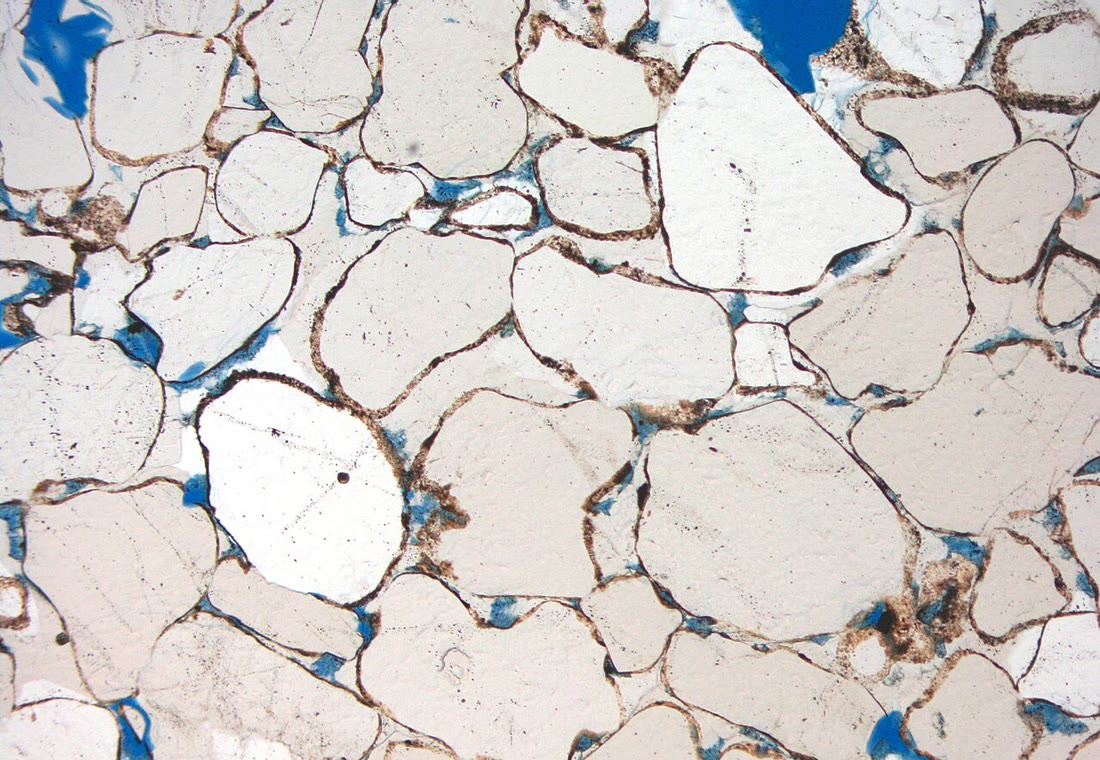
\includegraphics[width=0.62\linewidth]{images/book3/b1-quartz-overgrowths.jpg}

{\small Una \omterm{def:b1:field-lab-methods-1:thin-section}{lámina delgada} de arenisca de cuarzo, la arenisca de Potsdam (Cámbrico) del estado de Nueva York, con \omterm{def:b1:field-lab-methods-1:microscope}{luz polarizada plana}. Los granos detríticos redondeados están delineados por bordes
oscuros de polvo y arcilla; el cuarzo transparente fuera de los bordes es el \omterm{def:b1:diagenesis-basins:cement}{cemento} que creció sobre los granos, en continuidad óptica con ellos, hasta que los recrecimientos vecinos se encontraron
a lo largo de caras rectas. Resina azul rellena lo que queda de los poros. (M.~C.~Rygel, CC~BY-SA~4.0, a través de Wikimedia Commons; barra de escala del original recortada.)}
\label{fig:b1:diagenesis-basins:overgrowths}
\end{omfigure}
% ledger: commons:potsdam

No todos los cambios destruyen porosidad. El agua subsaturada en un \omterm{def:b1:rock-forming-minerals:mineral}{mineral} lo disuelve: granos de \omterm{def:b1:rock-forming-minerals:groups}{feldespato} y de carbonato, y \omterm{def:b1:diagenesis-basins:cement}{cementos} carbonatados anteriores, pueden eliminarse y dejar una
porosidad secundaria, poros con la forma de los granos que reemplazan. Los \omterm{def:b1:rock-forming-minerals:mineral}{minerales} de arcilla crecen a su vez en los poros, como revestimientos de los granos o como cristales que rellenan los poros
y estrechan los pasos entre ellos, reduciendo la permeabilidad. También cambian los \omterm{def:b1:rock-forming-minerals:mineral}{minerales} del sedimento: la aragonita de las conchas y de la \omterm{def:b1:chemical-biogenic-sediments:factory}{fábrica de carbonato} vuelve a calcita, que es estable en la
superficie, y la calcita en presencia de agua con magnesio puede convertirse en dolomita.
% ledger: og:diagenesis

La sustitución de calcita por dolomita, la dolomitización, es una reacción con el magnesio del agua,
\[
  \ce{2 CaCO3 + Mg^2+ -> CaMg(CO3)2 + Ca^2+},
\]
y cambia el volumen del sólido.

\begin{proposition}[La dolomitización crea porosidad]\label{prop:b1:diagenesis-basins:dolomite}
Si dos moles de calcita de densidad $\rho_c$ se reemplazan por un mol de dolomita de densidad $\rho_d$, el volumen del sólido disminuye en la fracción
\[
  1 - \frac{M_d/\rho_d}{2M_c/\rho_c},
\]
donde $M_c$ y $M_d$ son las masas molares. Con $\rho_c = \qty{2.71}{g.cm^{-3}}$ y $\rho_d = \qty{2.84}{g.cm^{-3}}$ esta fracción es de \qty{12.1}{\percent}.
\end{proposition}

\begin{proof}
El volumen molar de un \omterm{def:b1:rock-forming-minerals:mineral}{mineral} es su masa molar dividida por su densidad. Dos moles de calcita ocupan $2M_c/\rho_c$ y un mol de dolomita $M_d/\rho_d$; la fracción perdida es uno menos su cociente. Con
$M_c = \qty{100.09}{g.mol^{-1}}$ y $M_d = \qty{184.40}{g.mol^{-1}}$ los dos volúmenes son
$2\times\qty{36.93}{cm^3} = \qty{73.86}{cm^3}$ y \qty{64.93}{cm^3}, y $1 - 64.93/73.86 = \num{0.121}$.
\end{proof}

Si el volumen externo de la roca no cambia, el sólido perdido es espacio poroso ganado: una caliza de porosidad \num{0.10} reemplazada mol a mol por dolomita tiene una porosidad de unos \num{0.21}.
La reacción necesita mucho magnesio, que el agua de mar contiene en unos \qty{1.28}{g} por kilogramo; se favorece donde salmueras o agua de mar fluyen durante mucho tiempo a través de la roca
(\cref{exo:b1:diagenesis-basins:12}).
% ledger: hom:calcite, webmineral:others, teos10:reference-composition, teos10:reference-salinity

La \omterm{def:b1:diagenesis-basins:diagenesis}{diagénesis} sigue la historia del sedimento. Justo después del depósito, cerca de la superficie, el agua de poros es todavía la del mar, el lago o la lluvia: los sedimentos están bioturbados, se
cementan pronto en el fondo marino o en el suelo, y la aragonita se convierte en calcita. Con el enterramiento y el calentamiento dominan la \omterm{def:b1:diagenesis-basins:compaction}{compactación}, la disolución por presión y el \omterm{def:b1:diagenesis-basins:cement}{cemento} de cuarzo.
Si la cuenca se levanta y se erosiona después, el agua dulce de la superficie vuelve a entrar en las rocas y disuelve de nuevo carbonato y \omterm{def:b1:rock-forming-minerals:groups}{feldespato}. Una \omterm{def:b1:field-lab-methods-1:thin-section}{lámina delgada} registra el orden de estos
sucesos: un \omterm{def:b1:diagenesis-basins:cement}{cemento} que rellena el poro dejado por un grano disuelto es más joven que la disolución, y un recrecimiento roto por la \omterm{def:b1:diagenesis-basins:compaction}{compactación} es más antiguo que la \omterm{def:b1:diagenesis-basins:compaction}{compactación}.

\section{Cuencas sedimentarias}\label{sec:b1:diagenesis-basins:basins}

El sedimento de kilómetros de espesor solo se acumula donde el suelo sigue hundiéndose.

\begin{definition}[Cuenca sedimentaria]\label{def:b1:diagenesis-basins:basin}
Una \emph{cuenca sedimentaria}\index{cuenca sedimentaria} es una región de la superficie de la Tierra donde la \omterm{def:b1:layered-earth:layers}{corteza} se ha hundido durante mucho tiempo, de unos pocos millones a unos pocos cientos de millones de años, y donde el espacio así creado se ha llenado de sedimento, de cientos de metros a muchos kilómetros de espesor.
\end{definition}

\begin{definition}[Hundimiento, hundimiento tectónico]\label{def:b1:diagenesis-basins:subsidence}
El \emph{hundimiento}\index{hundimiento} de una cuenca es el movimiento hacia abajo de su basamento, la superficie sobre la que descansan sus sedimentos, medido respecto de una referencia fija como el centro de la Tierra. Su
\emph{hundimiento tectónico}\index{hundimiento tectónico} es la parte debida a los procesos que forman la cuenca, distinta del hundimiento adicional causado por el peso de los sedimentos y del agua que la llenan; se mide por el hundimiento que el basamento habría tenido bajo el agua sola.
\end{definition}

Lo que hace hundirse el suelo es el emplazamiento de la cuenca en la placa (figura de abajo).

\begin{description}
  \item[Cuencas de rift.] Las \omterm{def:b1:faults-folds-fabrics:fault-types}{fallas normales} estiran la \omterm{def:b1:layered-earth:layers}{corteza}, y entre ellas bajan bloques (\cref{ch:b1:rifts-ridges-margins}). Las cuencas son estrechas y asimétricas, semigrábenes que se llenan más deprisa junto a su falla de borde. Los yacimientos petrolíferos del mar del Norte yacen en las estructuras de sus grábenes de Viking y Central, enterrados bajo sedimentos más jóvenes. Cuando cesa el estiramiento, la \omterm{def:b1:layered-earth:lithosphere}{litosfera} adelgazada y calentada se enfría, se contrae y sigue hundiéndose, despacio, durante decenas de millones de años. El centro del mar del Norte, cuyo último gran estiramiento terminó a mitad del Cretácico, se hundió entonces como una cuenca amplia en forma de platillo, llenada sucesivamente por creta, areniscas y, durante gran parte del Terciario, lutitas y lodolitas; su basamento, cargado solo por el agua, se habría hundido \qtyrange{1100}{1400}{m} en el centro.
  \item[Márgenes pasivos.] Donde el rift se convirtió en océano, el mismo enfriamiento hace que cada margen se hunda tras la ruptura, y una cuña de sedimento que se engruesa hacia el océano se construye sobre las antiguas cuencas de rift.
  \item[Cuencas de antepaís.] Delante de un cinturón de \omterm{def:b1:faults-folds-fabrics:fault-types}{cabalgamientos}, el peso de las láminas de \omterm{def:b1:faults-folds-fabrics:fault-types}{cabalgamiento} apiladas dobla la \omterm{def:b1:layered-earth:lithosphere}{litosfera} hacia abajo, por \omterm{def:b1:isostasy-gravity:isostasy}{isostasia}, formando una cuenca más profunda junto al cinturón y llena de los derrubios erosionados de él. La mayor parte de las rocas cretácicas del oeste de Canadá se depositaron en una cuenca así, delante de las Montañas Rocosas.
  \item[Cuencas intracratónicas.] En el interior de los continentes viejos, lejos de cualquier límite de placa, regiones amplias, redondas u ovaladas se han hundido despacio durante tiempos muy largos. La cuenca de París es el centro de una depresión estructural así, entre los viejos macizos de Bretaña, el Macizo Central y los Vosgos y las Ardenas.
  \item[Cuencas de desgarre.] Donde una \omterm{def:b1:faults-folds-fabrics:fault-types}{falla de desgarre} da un paso lateral en el sentido que separa sus paredes --- una curvatura de liberación ---, un paralelogramo de \omterm{def:b1:layered-earth:layers}{corteza} se hunde entre los dos ramales de la falla: una cuenca de tipo pull-apart, como las de la región de Los Ángeles a lo largo del sistema de San Andrés.
\end{description}
% ledger: ws:basins, sc80:north-sea, britannica:paris-basin

La razón por la que la \omterm{def:b1:layered-earth:lithosphere}{litosfera} se hunde en cada situación, a qué velocidad, y cómo se comparan las cuencas, es el tema del volumen del año~2; aquí se distinguen por dónde yacen y por la forma de su relleno.

\begin{omfigure}
\begin{tikzpicture}[font=\scriptsize, line join=round]
% (a) rift: a half-graben
\begin{scope}
  \fill[lith granite] (0,0) -- (0,1.6) -- (1.4,1.6) -- (2.2,0.2) -- (5.0,1.0) -- (5.0,0) -- cycle;
  \fill[lith shale] (1.4,1.6) -- (2.2,0.2) -- (5.0,1.0) -- (5.0,1.6) -- cycle;
  \fill[lith sandstone] (1.4,1.6) -- (1.75,0.99) -- (5.0,1.25) -- (5.0,1.6) -- cycle;
  \draw[normal fault, thick] (1.4,1.6) -- (2.3,0.0);
  \draw[black!70] (0,1.6) -- (5.0,1.6);
  \node[anchor=south west] at (0,1.65) {(a) rift: un semigraben};
  \node[fill=white, fill opacity=0.8, text opacity=1, inner sep=1pt] at (3.9,0.3) {basamento};
  \node[fill=white, fill opacity=0.8, text opacity=1, inner sep=1pt] at (0.65,0.8) {bloque yacente};
\end{scope}
% (b) passive margin: a seaward-thickening wedge over thinned crust
\begin{scope}[xshift=6.6cm]
  \fill[lith sea] (2.0,1.6) -- (5.0,1.6) -- (5.0,0.75) -- (3.6,0.95) -- cycle;
  \fill[lith granite] (0,0) -- (0,1.2) -- (2.0,1.0) -- (3.6,0.35) -- (5.0,0.05) -- (5.0,0) -- cycle;
  \fill[lith shale] (0,1.2) -- (2.0,1.0) -- (3.6,0.35) -- (5.0,0.05) -- (5.0,0.75) -- (3.6,0.95) -- (2.0,1.6) -- (0,1.6) -- cycle;
  \draw[black!70] (0,1.6) -- (2.0,1.6) -- (3.6,0.95) -- (5.0,0.75);
  \draw[blue!60!black, thick] (2.0,1.6) -- (5.0,1.6);
  \node[anchor=south west] at (0,1.65) {(b) margen pasivo};
  \node[fill=white, fill opacity=0.8, text opacity=1, inner sep=1pt] at (1.0,0.45) {corteza continental adelgazada};
  \node[anchor=north east] at (5.0,1.58) {océano};
\end{scope}
% (c) foreland basin: asymmetric, deepest against the thrust belt
\begin{scope}[yshift=-3.3cm]
  \fill[lith granite] (0,0) -- (0,0.55) -- (5.0,1.35) -- (5.0,0) -- cycle;
  \fill[lith sandstone] (0,0.55) -- (5.0,1.35) -- (5.0,1.6) -- (0,1.6) -- cycle;
  \fill[lith conglomerate] (1.0,1.6) -- (3.6,1.6) -- (1.0,1.0) -- cycle;
  \fill[omLithSchist, draw=black!70] (0,0.95) -- (1.9,1.6) -- (1.3,1.95) -- (0.4,2.25) -- (0,2.3) -- cycle;
  \draw[thrust fault] (0,0.95) -- (1.9,1.6);
  \draw[thrust fault] (0,1.55) -- (1.15,1.95);
  \draw[black!70] (1.9,1.6) -- (5.0,1.6);
  \node[anchor=south west] at (2.0,1.65) {(c) cuenca de antepaís};
  \node[anchor=south west, inner sep=1pt] at (0.25,2.3) {cinturón de cabalgamientos};
  \node[fill=white, fill opacity=0.8, text opacity=1, inner sep=1pt] at (3.9,0.35) {basamento};
\end{scope}
% (d) intracratonic basin: a broad sag, layers thickening to the centre
\begin{scope}[xshift=6.6cm, yshift=-3.3cm]
  \fill[lith granite] (0,0) -- (0,1.5) .. controls (1.6,1.1) and (2.0,0.3) .. (2.5,0.3) .. controls (3.0,0.3) and (3.4,1.1) .. (5.0,1.5) -- (5.0,0) -- cycle;
  \fill[lith limestone] (0,1.5) .. controls (1.6,1.1) and (2.0,0.3) .. (2.5,0.3) .. controls (3.0,0.3) and (3.4,1.1) .. (5.0,1.5) -- (5.0,1.6) -- (0,1.6) -- cycle;
  \fill[lith shale] (0.6,1.6) .. controls (1.6,1.35) and (2.1,0.85) .. (2.5,0.85) .. controls (2.9,0.85) and (3.4,1.35) .. (4.4,1.6) -- cycle;
  \fill[lith sandstone] (1.3,1.6) .. controls (1.9,1.5) and (2.2,1.3) .. (2.5,1.3) .. controls (2.8,1.3) and (3.1,1.5) .. (3.7,1.6) -- cycle;
  \draw[black!70] (0,1.6) -- (5.0,1.6);
  \node[anchor=south west] at (0,1.65) {(d) cuenca intracratónica};
  \node[fill=white, fill opacity=0.8, text opacity=1, inner sep=1pt] at (4.2,0.4) {basamento};
\end{scope}
\end{tikzpicture}

{\small Cuatro tipos de \omterm{def:b1:diagenesis-basins:basin}{cuenca sedimentaria} en corte transversal (esquemáticos, no a escala; escala vertical exagerada). (a)~Un rift: el relleno se engruesa junto a la falla de borde de un
\omterm{def:b1:rifts-ridges-margins:rift}{semigraben}. (b)~Un \omterm{def:b1:rifts-ridges-margins:passive-margin}{margen pasivo}: una cuña de sedimento que se engruesa hacia el océano sobre la \omterm{def:b1:layered-earth:layers}{corteza} continental adelgazada. (c)~Una cuenca de antepaís, más profunda junto al cinturón de
\omterm{def:b1:faults-folds-fabrics:fault-types}{cabalgamientos} cuyo peso la dobla hacia abajo, y alimentada por sus derrubios, los más gruesos (conglomerado) cerca del cinturón; el cinturón cabalga sobre el borde de su propia cuenca. (d)~Una cuenca
intracratónica: una depresión amplia cuyas capas se engruesan hacia el centro.}
\label{fig:b1:diagenesis-basins:types}
\end{omfigure}

\begin{inthefield}[Cómo se conocen las cuencas]
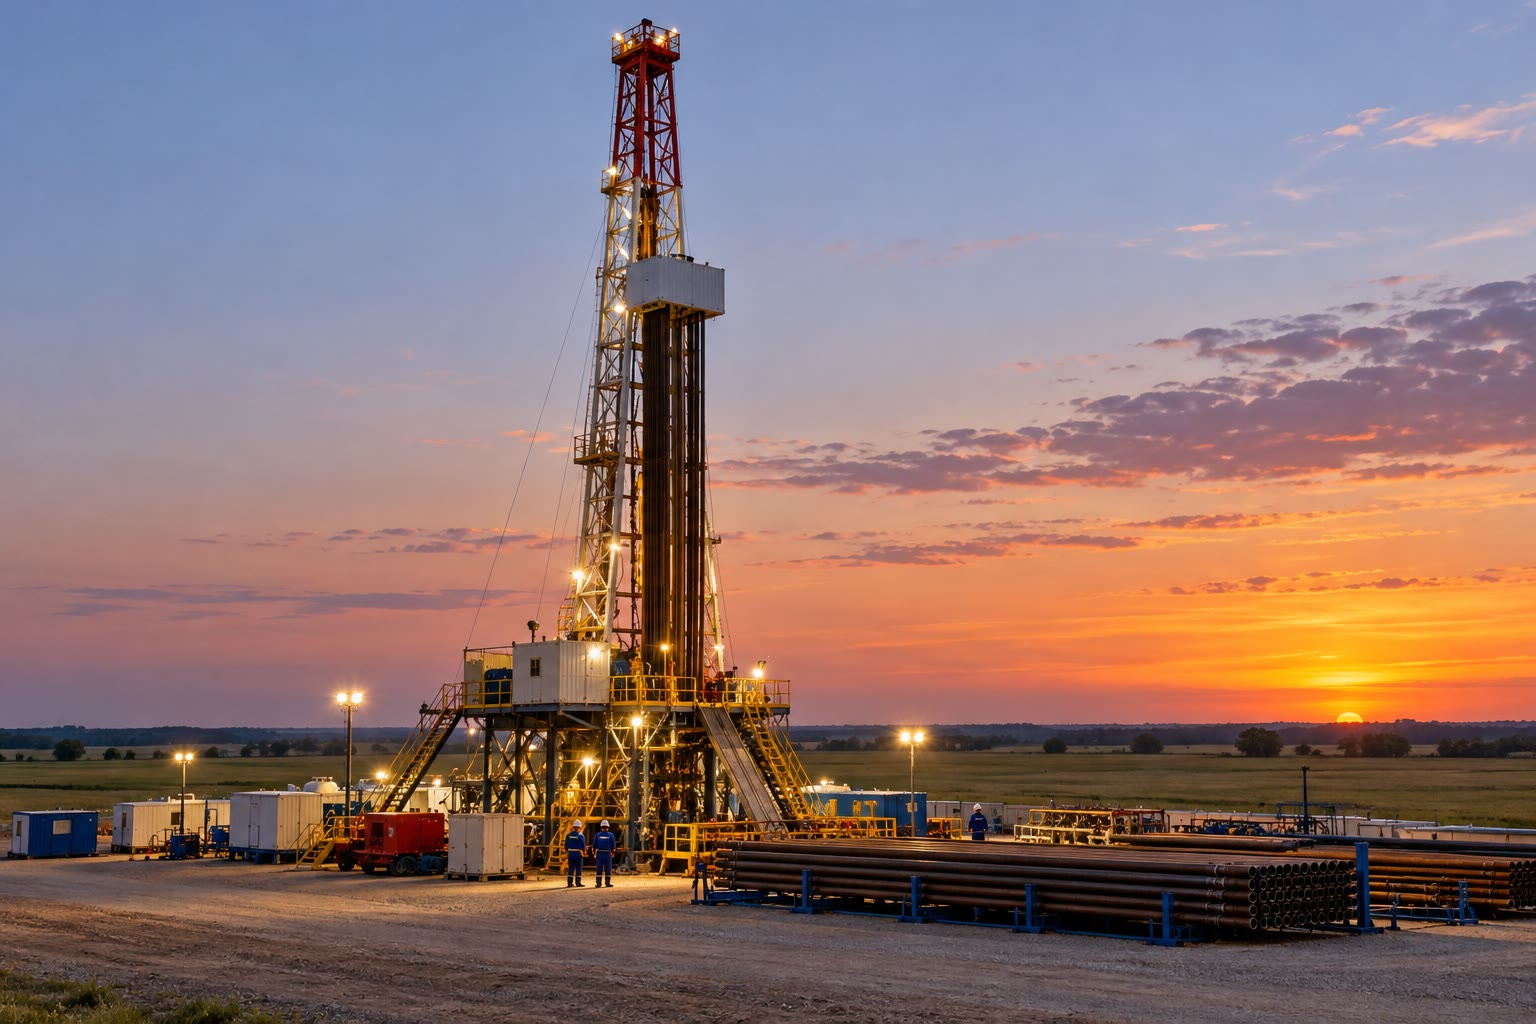
\includegraphics[width=0.3\linewidth]{images/book3/ai/b1-drilling-rig.jpg}\hfill
\begin{minipage}[b]{0.67\linewidth}
Casi todo lo que se sabe del relleno profundo de una cuenca procede de la búsqueda de petróleo, gas y agua. Los levantamientos de reflexión sísmica dibujan sus capas y sus fallas
sobre miles de kilómetros cuadrados; los pozos la muestrean en un punto. Un pozo devuelve los recortes de roca cortados por la broca, a intervalos testigos, y registros continuos de las
propiedades físicas de las rocas alrededor del sondeo, a partir de los cuales se lee la porosidad metro a metro. Las curvas porosidad--profundidad de la \omterm{prop:b1:diagenesis-basins:athy}{ley de Athy}, y las historias de
\omterm{def:b1:diagenesis-basins:subsidence}{hundimiento} de las cuencas, se construyeron por primera vez a partir de tales pozos.
\end{minipage}

\smallskip
{\small Una torre de perforación terrestre al atardecer, con la tubería apilada en los bastidores en primer plano (ilustración IA).}
\end{inthefield}
% ledger: sc80:north-sea

\section{Hundimiento, espacio de acomodación y nivel del mar}\label{sec:b1:diagenesis-basins:accommodation}

El sedimento solo puede acumularse donde hay sitio para él por debajo del nivel al que sería trasladado. En el mar ese nivel está cerca del nivel del mar, y el sitio es cuestión de dos
movimientos: el del fondo y el de la superficie del mar.

\begin{definition}[Espacio de acomodación]\label{def:b1:diagenesis-basins:accommodation}
El \emph{espacio de acomodación}\index{espacio de acomodación} en un punto de una cuenca es el espacio disponible para que se acumule sedimento allí: la distancia vertical desde la cima del
sedimento hasta el nivel del mar, el nivel de base de la sedimentación marina. El espacio de acomodación creado en un intervalo de tiempo es el aumento de la distancia desde un dato unido al
basamento hasta el nivel del mar.
\end{definition}

\begin{definition}[Eustasia, nivel relativo del mar]\label{def:b1:diagenesis-basins:eustasy}
La \emph{eustasia}\index{eustasia} es el cambio del nivel del océano mundial medido respecto de una referencia fija, el centro de la Tierra, causado por un cambio en el volumen de agua del océano
o en el volumen de las cuencas oceánicas; es la misma en todas partes. El \emph{nivel relativo del mar}\index{nivel relativo del mar} en un lugar es la altura de la superficie del mar sobre
un dato unido al basamento allí; cambia por eustasia y por el movimiento vertical del terreno.
\end{definition}

\begin{proposition}[El balance del espacio de acomodación]\label{prop:b1:diagenesis-basins:budget}
En un intervalo de tiempo, sea $\Delta E$ la subida eustática del nivel del mar y $S$ el \omterm{def:b1:diagenesis-basins:subsidence}{hundimiento} del basamento (ambos positivos hacia arriba para el mar, hacia abajo para el suelo). El \omterm{def:b1:diagenesis-basins:accommodation}{espacio
de acomodación} creado es
\[
  \Delta A = \Delta E + S ,
\]
y se reparte entre el espesor de sedimento añadido por encima del dato, $\Delta T$, y la profundización del agua, $\Delta W$: $\Delta E + S = \Delta T + \Delta W$.
\end{proposition}

\begin{proof}
Mídanse las alturas desde la referencia fija. Sea $e$ la altura de la superficie del mar, $b$ la del dato, $T$ el espesor de sedimento por encima del dato, y $W$ la profundidad del agua
encima del sedimento, de modo que $e = b + T + W$. El \omterm{def:b1:diagenesis-basins:eustasy}{nivel relativo del mar} es $R = e - b = T + W$. Durante el intervalo, $\Delta e =
\Delta E$ y $\Delta b = -S$, así que $\Delta R = \Delta E + S$; y $\Delta R =
\Delta T + \Delta W$.
\end{proof}

Un fondo marino que se mantiene a profundidad constante ($\Delta W = 0$) se llena exactamente tan deprisa como se crea el \omterm{def:b1:diagenesis-basins:accommodation}{espacio de acomodación}; uno que se vuelve más somero se llena más deprisa,
y la línea de costa avanza mar adentro; uno que se profundiza se queda sin sedimento. $\Delta T$ es el cambio de espesor de toda la pila por encima del dato: cuenta el sedimento nuevo depositado,
menos el adelgazamiento de los sedimentos más antiguos debajo a medida que se compactan, así que la propia \omterm{def:b1:diagenesis-basins:compaction}{compactación} crea espacio para más sedimento (figura de abajo).

\begin{omfigure}
\begin{tikzpicture}[font=\footnotesize, >=Stealth]
\def\col#1#2#3#4#5{% x, datum, sediment top, sea, label
  \fill[lith granite] (#1,0.2) rectangle ++(1.4,#2-0.2);
  \fill[lith shale] (#1,#2) rectangle ++(1.4,#3-#2);
  \fill[lith sea] (#1,#3) rectangle ++(1.4,#4-#3);
  \draw[black!70] (#1,#2) -- ++(1.4,0);
  \draw[blue!60!black, thick] (#1-0.2,#4) -- ++(1.8,0);
  \node[anchor=north] at (#1+0.7,0.15) {#5};}
\draw[black!60, dash dot] (-0.6,0.9) -- (8.6,0.9) node[anchor=west, align=left] {referencia\\ fija};
\col{0}{1.5}{3.0}{3.6}{tiempo $t_1$}
\col{4.4}{1.0}{3.4}{3.9}{tiempo $t_2$}
% eustasy
\draw[<->, omThm] (3.0,0.9) -- (3.0,3.6) node[midway, fill=white, inner sep=1pt] {$e_1$};
\draw[<->, omThm] (7.4,0.9) -- (7.4,3.9) node[midway, fill=white, inner sep=1pt] {$e_2$};
% subsidence of the datum
\draw[dashed, black!60] (1.4,1.5) -- (4.4,1.5);
\draw[->, thick] (4.2,1.5) -- (4.2,1.0) node[midway, anchor=east] {$S$};
% relative sea level
\draw[<->] (-0.35,1.5) -- (-0.35,3.6) node[midway, anchor=east] {$R_1$};
\draw[<->] (6.05,1.0) -- (6.05,3.9) node[midway, anchor=west] {$R_2$};
\node[anchor=west] at (1.5,2.25) {$T_1$};
\node[anchor=west] at (1.5,3.3) {$W_1$};
\node at (5.1,2.2) {$T_2$};
\node at (5.1,3.65) {$W_2$};
\node[anchor=south, align=center, blue!60!black] at (5.1,3.95) {nivel del mar};
\node[anchor=west, align=left, font=\scriptsize] at (8.6,2.4) {$R = e - b = T + W$\\[2pt] $\Delta R = \Delta E + S$\\ $\phantom{\Delta R} = \Delta T + \Delta W$};
\end{tikzpicture}

{\small \omterm{def:b1:diagenesis-basins:accommodation}{Espacio de acomodación} en un lugar en dos momentos (esquemático). Entre $t_1$ y $t_2$ el nivel del mar sube $\Delta E = e_2 - e_1$ por encima de la referencia fija, y el basamento se hunde
$S$: el \omterm{def:b1:diagenesis-basins:eustasy}{nivel relativo del mar} $R$ crece en $\Delta E + S$, el \omterm{def:b1:diagenesis-basins:accommodation}{espacio de acomodación} creado, que se reparte entre más sedimento ($T_2 > T_1$) y un cambio de la profundidad del agua (aquí un ligero
ascenso, $W_2 < W_1$).}
\label{fig:b1:diagenesis-basins:accommodation}
\end{omfigure}

Una cuenca no se hunde solo por su \omterm{def:b1:diagenesis-basins:subsidence}{hundimiento tectónico}: el sedimento que la llena es una carga, y la \omterm{def:b1:layered-earth:lithosphere}{litosfera} se hunde más bajo ella.

\begin{proposition}[La carga de sedimento amplifica el hundimiento]\label{prop:b1:diagenesis-basins:loading}
En \omterm{def:b1:isostasy-gravity:isostasy}{isostasia} local (de Airy) sobre un \omterm{def:b1:layered-earth:layers}{manto} de densidad $\rho_m$, una cuenca cuyo basamento, cargado solo por agua de densidad $\rho_w$, yacería a la profundidad $Y$
bajo el nivel del mar, contiene, cuando se llena hasta el nivel del mar con sedimento de densidad media
$\rho_s$, el espesor
\[
  h = Y\,\frac{\rho_m - \rho_w}{\rho_m - \rho_s}
\]
de sedimento. En tierra, llenada hasta el nivel de los alrededores con aire encima, el factor es $\rho_m/(\rho_m - \rho_s)$.
\end{proposition}

\begin{proof}
Compárense las dos columnas con la misma \omterm{def:b1:layered-earth:lithosphere}{litosfera}, de masa $M$ por unidad de área y espesor $L$, hasta una \omterm{def:b1:isostasy-gravity:isostasy}{profundidad de compensación} $z_c$ por debajo de ambas. La columna cargada por agua
contiene $\rho_w Y + M + \rho_m(z_c - Y - L)$; la llena de sedimento, $\rho_s h + M + \rho_m(z_c - h - L)$. Por
\cref{prop:b1:isostasy-gravity:equal-mass} las dos masas son iguales, así que
$\rho_w Y - \rho_m Y = \rho_s h - \rho_m h$, es decir $h(\rho_m - \rho_s) =
Y(\rho_m - \rho_w)$. Con aire en lugar de agua, $\rho_w$ se sustituye por cero.
\end{proof}

Con $\rho_m = \qty{3300}{kg.m^{-3}}$, $\rho_w = \qty{1030}{kg.m^{-3}}$ y un sedimento de densidad media \qty{2300}{kg.m^{-3}}, el factor es
$2270/1000 = \num{2.27}$: una cuenca cuyo \omterm{def:b1:diagenesis-basins:subsidence}{hundimiento tectónico} daría espacio para \qty{1}{km} de agua contiene \qty{2.27}{km} de sedimento. En tierra el factor sería
$3300/1000 = \num{3.3}$. La densidad del relleno no es constante: crece a medida que el sedimento se compacta, y con ella el factor, de modo que convertir un espesor de sedimento
en un \omterm{def:b1:diagenesis-basins:subsidence}{hundimiento tectónico} exige descompactar cada capa, paso de tiempo a paso de tiempo. Ese procedimiento, el retrodesplazamiento (backstripping), pertenece al volumen del año~2.

El nivel del mar en sí mismo está lejos de ser fijo. En el Máximo Glacial, los \omterm{def:b1:layered-earth:layers}{mantos} de hielo cubrían buena parte de Norteamérica y del norte de Europa, y el agua inmovilizada en ellos se había
tomado del océano. Corregidas por la respuesta de la Tierra sólida a las cargas cambiantes de hielo y de agua, las observaciones de antiguas líneas de costa dan un nivel del mar que bajó deprisa
unos \qty{40}{m} hace unos \num{30000} años, y luego despacio, hasta \qty{134}{m} por debajo del actual, entre \qtyrange{29}{21}{\ka}; el hielo asentado contenía entonces unos \qty{52e6}{km^3} más que hoy.
La cifra de \qty{125}{m} que se cita a menudo es menor porque no suele corregirse por estos efectos isostáticos. La deglaciación llegó sobre todo entre hace unos \qty{16.5}{\ka} y \qty{8.2}{\ka}, a una media de
\qty{12}{m} por mil años, y a \qty{40}{mm} al año o más entre \qty{14.5}{\ka} y \qty{14.0}{\ka}.
% ledger: lambeck:lgm, lambeck:deglaciation

Los niveles bajos más antiguos se leen en los isótopos de oxígeno de los foraminíferos de los testigos de fondo marino, que registran el volumen de hielo en tierra. Apilando siete de tales
reconstrucciones a lo largo de los últimos \num{430000} años, y cinco a lo largo de los últimos \num{800000}, se promedian los errores de cada una; escalada al Holoceno y al último nivel bajo glacial, la pila lleva
una incertidumbre de \qtyrange{9}{12}{m} (figura de abajo). Muestra los ciclos glaciales como un diente de sierra: caídas lentas del nivel del mar, cada una terminada por una subida rápida ---cinco veces en los
últimos \num{800000} años, una subida de más de \qty{100}{m} en menos de \num{20000} años. La \omterm{def:b1:diagenesis-basins:eustasy}{eustasia} a esta escala mueve la línea de costa de un lado a otro de las plataformas continentales.
% ledger: spratt:stack, data:b3-sealevel-stack

\begin{omfigure}
\begin{tikzpicture}[font=\footnotesize]
\begin{axis}[width=16cm, height=4.8cm, xmin=0, xmax=800, ymin=-150, ymax=40,
    x dir=reverse, xlabel={edad (miles de años antes del presente)}, xlabel style={yshift=2pt},
    ylabel={nivel del mar (m)}, ytick={-150,-100,-50,0},
    title={(a) los últimos \num{800000} años (cinco registros)}, title style={font=\footnotesize},
    axis on top]
  \addplot[draw=none, name path=hi] table[x=age, y=hi] {figdata/out/bachelor-1-sea_level-long.dat};
  \addplot[draw=none, name path=lo] table[x=age, y=lo] {figdata/out/bachelor-1-sea_level-long.dat};
  \addplot[omThm!25] fill between[of=hi and lo];
  \addplot[thin, omThm] table[x=age, y=sl] {figdata/out/bachelor-1-sea_level-long.dat};
  \draw[black!50, densely dotted] (axis cs:0,0) -- (axis cs:800,0);
\end{axis}
\end{tikzpicture}

\medskip
\begin{tikzpicture}[font=\footnotesize]
\begin{axis}[width=16cm, height=4.8cm,
    xmin=0, xmax=140, ymin=-160, ymax=40, x dir=reverse,
    xlabel={edad (miles de años antes del presente)}, ylabel={nivel del mar (m)},
    ytick={-150,-100,-50,0},
    title={(b) los últimos \num{140000} años (siete registros)}, title style={font=\footnotesize},
    axis on top]
  \addplot[draw=none, name path=hi] table[x=age, y=hi] {figdata/out/bachelor-1-sea_level-short.dat};
  \addplot[draw=none, name path=lo] table[x=age, y=lo] {figdata/out/bachelor-1-sea_level-short.dat};
  \addplot[omThm!25] fill between[of=hi and lo];
  \addplot[thick, omThm] table[x=age, y=sl] {figdata/out/bachelor-1-sea_level-short.dat};
  \draw[black!50, densely dotted] (axis cs:0,0) -- (axis cs:140,0);
  \addplot[only marks, mark=*, mark size=1.6pt, black] coordinates {(21,-134)};
  \draw[black!60, thin] (axis cs:21,-131) -- (axis cs:21,-46);
  \node[anchor=south, font=\scriptsize, fill=white, inner sep=1pt] at (axis cs:36,-46) {\qty{-134}{m} a \qty{21}{\ka}, según antiguas líneas de costa (Lambeck et al.\ 2014)};
\end{axis}
\end{tikzpicture}

{\small Nivel global del mar respecto de hoy, según la pila de Spratt y Lisiecki (2016): la primera componente principal de cinco reconstrucciones a partir de testigos de fondo marino a lo largo de
\num{800000} años (a) y de siete a lo largo de los últimos \num{140000} (b), con su banda de una desviación típica. El valor más bajo de la pila, \qty{-130}{m} a \qty{24}{\ka}, yace dentro de esa banda
de los \qty{-134}{m} hallados a partir de antiguas líneas de costa (punto); el último interglaciar está unos \qty{3}{m} por encima de hoy a \qty{121}{\ka}. Datos: NOAA NCEI World Data Service for Paleoclimatology.}
\label{fig:b1:diagenesis-basins:sea-level}
\end{omfigure}
% computed in figdata/bachelor-1/sea_level.py; ledger: data:b3-sealevel-stack, spratt:stack, lambeck:lgm

A lo largo de la vida de una cuenca tales oscilaciones son breves. Una caída glacial de más de \qty{100}{m} en unas pocas decenas de miles de años es rápida y grande comparada con el \omterm{def:b1:diagenesis-basins:subsidence}{hundimiento
tectónico}, que suma un kilómetro o más solo a lo largo de decenas de millones de años; pero las oscilaciones glaciales se mantienen dentro de un rango de unos \qty{150}{m}, así que, en el relleno grueso
de una cuenca, el \omterm{def:b1:diagenesis-basins:subsidence}{hundimiento} aporta la mayor parte del espacio, y la \omterm{def:b1:diagenesis-basins:eustasy}{eustasia} marca el ritmo de sus capas.
% ledger: data:b3-sealevel-stack, sc80:north-sea

\section{Ejercicios}

\begin{exercise}[$\star$]\label{exo:b1:diagenesis-basins:1}
Con los parámetros de \cref{tab:b1:diagenesis-basins:athy}, calcúlense las porosidades de la arenisca y de la lutita a \qty{2000}{m}. ¿A qué profundidad ha bajado la porosidad de cada una a la mitad de su valor superficial?
% ledger: pybacktrack:compaction
\end{exercise}

\begin{exercise}[$\star$]\label{exo:b1:diagenesis-basins:2}
Durante un intervalo de tiempo, el nivel del mar sube \qty{30}{m} por \omterm{def:b1:diagenesis-basins:eustasy}{eustasia}, el basamento de una plataforma se hunde \qty{50}{m}, y se añaden \qty{60}{m} de sedimento por encima de un dato
sobre el basamento. Con \cref{prop:b1:diagenesis-basins:budget}, calcúlense el \omterm{def:b1:diagenesis-basins:accommodation}{espacio de acomodación} creado y el cambio de la profundidad del agua. ¿Se profundiza o se hace más somera la plataforma?
\end{exercise}

\begin{exercise}[$\star$]\label{exo:b1:diagenesis-basins:3}
El \omterm{def:b1:diagenesis-basins:subsidence}{hundimiento tectónico} de una cuenca daría espacio para \qty{1.0}{km} de agua. Con $\rho_m = \qty{3300}{kg.m^{-3}}$ y $\rho_w = \qty{1030}{kg.m^{-3}}$, ¿qué espesor tiene el sedimento que la llena hasta el
nivel del mar si su densidad media es de \qty{2300}{kg.m^{-3}}? ¿Y de \qty{2500}{kg.m^{-3}}? ¿Por qué un relleno más denso da uno más grueso?
\end{exercise}

\begin{exercise}[$\star$]\label{exo:b1:diagenesis-basins:4}
La calcita tiene la masa molar \qty{100.09}{g.mol^{-1}} y la densidad \qty{2.71}{g.cm^{-3}}; la dolomita, \qty{184.40}{g.mol^{-1}} y \qty{2.84}{g.cm^{-3}}. (a)~Calcúlese el volumen molar de cada una.
(b)~¿En qué fracción cambia el volumen del sólido cuando dos moles de calcita se convierten en un mol de dolomita? (c)~Una caliza de porosidad \num{0.10} se dolomitiza mol a mol sin cambio de su
volumen externo. ¿Cuál es su nueva porosidad?
% ledger: hom:calcite, webmineral:others
\end{exercise}

\begin{exercise}[$\star\star$]\label{exo:b1:diagenesis-basins:5}
Una lutita ocupa los primeros \qty{1000}{m} de una cuenca. (a)~Calcúlese su espesor sólido y su porosidad media. (b)~Se entierra hasta que su techo yace a \qty{2000}{m}. Usando
\cref{met:b1:diagenesis-basins:decompaction} con el techo desplazado hacia abajo en lugar de hacia arriba, hállese su nuevo espesor y su porosidad media. (c)~¿Cuánta agua ha
expulsado cada metro cuadrado de la lutita?
% ledger: pybacktrack:compaction
\end{exercise}

\begin{exercise}[$\star\star$]\label{exo:b1:diagenesis-basins:6}
Una arenisca yace entre \qty{2500}{m} y \qty{2800}{m}. (a)~Calcúlese su espesor sólido. (b)~Descompáctese hasta la superficie con \cref{met:b1:diagenesis-basins:decompaction}, escribiendo
cada paso de Newton desde $b_0 = \qty{300}{m}$. (c)~¿En qué factor la ha adelgazado el enterramiento?
% ledger: pybacktrack:compaction
\end{exercise}

\begin{exercise}[$\star\star$]\label{exo:b1:diagenesis-basins:7}
En el Máximo Glacial el hielo asentado contenía unos \qty{52e6}{km^3} más que hoy. Tómense la densidad del hielo \qty{916.7}{kg.m^{-3}}, la del agua de deshielo \qty{1000}{kg.m^{-3}}, y el
área del océano actual \qty{361.84e6}{km^2}. (a)~¿Qué descenso del nivel del mar representa este hielo? (b)~Compárese con los \qty{134}{m} hallados a partir de antiguas líneas de costa.
(c)~¿Qué área oceánica daría exactamente \qty{134}{m}, y por qué era menor el océano glacial?
% ledger: lambeck:lgm, iapws:ice-density, charette:ocean-volume
\end{exercise}

\begin{exercise}[$\star\star$]\label{exo:b1:diagenesis-basins:8}
La pila del nivel del mar da \qty{-98.1}{m} a \qty{16}{\ka} y \qty{-9.1}{m} a \qty{8}{\ka}. (a)~Calcúlese la tasa media de subida, en metros por mil años, y compárese con los \qty{12}{m} por mil
años hallados a partir de antiguas líneas de costa para la deglaciación principal. (b)~Entre \qty{14.5}{\ka} y \qty{14.0}{\ka} el nivel del mar subió a \qty{40}{mm} al año o más. ¿Cuántas veces es eso el
promedio, y cuánto subió el nivel del mar en esos quinientos años?
% ledger: data:b3-sealevel-stack, lambeck:deglaciation
\end{exercise}

\begin{exercise}[$\star\star$]\label{exo:b1:diagenesis-basins:9}
Una plataforma yace bajo \qty{20}{m} de agua. Su basamento se hunde a \qty{50}{m} por millón de años. (a)~Durante dos millones de años el nivel del mar baja \qty{40}{m} por \omterm{def:b1:diagenesis-basins:eustasy}{eustasia} mientras la
profundidad del agua se mantiene. ¿Cuánto \omterm{def:b1:diagenesis-basins:accommodation}{espacio de acomodación} se crea, y cuánto sedimento se añade? (b)~Luego el nivel del mar baja \qty{120}{m} en \num{20000} años, al comienzo de una glaciación,
y no se añade sedimento. ¿A qué altura sobre el nivel del mar queda el antiguo fondo marino al final?
\end{exercise}

\begin{exercise}[$\star\star\star$]\label{exo:b1:diagenesis-basins:10}
(a)~Demuéstrese que una capa de espesor $h$ a la profundidad $z$, delgada comparada con la longitud de desintegración $\lambda$, tiene al restaurarla a la superficie el espesor $h_0 \approx h\,(1 - \varphi(z))/(1 -
\varphi_0)$. (b)~Apliqúese a \qty{10}{m} de lutita a \qty{3000}{m}, y compárese con la \omterm{def:b1:diagenesis-basins:compaction}{descompactación} exacta, \qty{23.1}{m}. (c)~¿Por qué la aproximación es ligeramente demasiado grande?
% ledger: pybacktrack:compaction
\end{exercise}

\begin{exercise}[$\star\star\star$]\label{exo:b1:diagenesis-basins:11}
Una cuenca se llena hasta el nivel del mar con \qty{3000}{m} de lutita, compactada por la \omterm{prop:b1:diagenesis-basins:athy}{ley de Athy}, con sus poros llenos de agua de densidad \qty{1030}{kg.m^{-3}}. (a)~Calcúlense la porosidad media y la
densidad media del relleno. (b)~Con \cref{prop:b1:diagenesis-basins:loading} y $\rho_m =
\qty{3300}{kg.m^{-3}}$, calcúlense el factor de carga y el \omterm{def:b1:diagenesis-basins:subsidence}{hundimiento} con carga de agua que representa
el relleno. (c)~¿Por qué tomar la densidad de los granos, \qty{2700}{kg.m^{-3}}, daría un factor mucho mayor, y por qué sería erróneo?
% ledger: pybacktrack:compaction
\end{exercise}

\begin{exercise}[$\star\star\star$]\label{exo:b1:diagenesis-basins:12}
Un metro cúbico de caliza de porosidad \num{0.10} debe dolomitizarse por completo, mol a mol. El agua de mar contiene \qty{35.165}{g} de sal por kilogramo, de los cuales la fracción másica \num{0.0365} es
magnesio (\qty{24.305}{g.mol^{-1}}). (a)~¿Cuántos moles de calcita contiene el cubo (volumen molar de \cref{exo:b1:diagenesis-basins:4})? (b)~¿Cuántos moles de magnesio necesita la reacción?
(c)~¿Qué masa y qué volumen de agua de mar (\qty{1030}{kg.m^{-3}}) deben atravesar el cubo si cede todo su magnesio? (d)~¿Qué dice la respuesta sobre dónde se forma la dolomita?
% ledger: teos10:reference-composition, teos10:reference-salinity, hom:calcite
\end{exercise}

\section{Problema: descompactar el relleno de una cuenca}

\begin{problem}[{Problema de fin de semana --- qué espesor tenían los sedimentos de un pozo cuando se depositaron, y cómo se hizo sitio para ellos}]
\label{pb:b1:diagenesis-basins:1}
% values: calc/ch23.py; the well, its units, ages and the eustatic changes are invented
Un pozo perforado en una llanura costera, al nivel del mar, atraviesa tres unidades antes de llegar al basamento a \qty{3200}{m}:
\begin{center}
\begin{tabular}{llll}
\hline
unidad & litología & profundidad actual (m) & tiempo de depósito \\
\hline
1 & arenisca & 0--800     & \qtyrange{15}{0}{\Ma} \\
2 & lutita     & 800--2600  & \qtyrange{55}{15}{\Ma} \\
3 & creta     & 2600--3200 & \qtyrange{75}{55}{\Ma} \\
\hline
\end{tabular}
\end{center}
Tómense los parámetros de \cref{tab:b1:diagenesis-basins:athy}, agua de poros de densidad \qty{1030}{kg.m^{-3}}, $g = \qty{9.81}{m.s^{-2}}$, y supóngase que cada unidad se compactó
según la \omterm{prop:b1:diagenesis-basins:athy}{ley de Athy}, con su agua libre de escapar, a lo largo de toda su historia. Los microfósiles muestran que el agua era somera, y de la misma profundidad, al principio y al final de cada intervalo.

\medskip
\noindent\textbf{Parte I --- La columna hoy.}
\begin{enumerate}
  \item Calcúlese la porosidad en el techo y en la base de cada unidad.
  \item Calcúlese la porosidad media de cada unidad.
  \item ¿Cuánta agua contiene cada unidad bajo un metro cuadrado?
  \item Calcúlese la densidad aparente de cada unidad, saturada de agua, y la densidad media de toda la columna.
  \item Calcúlense las presiones litostática e hidrostática en la base de la columna, y el \omterm{def:b1:stress-strain-rheology:lithostatic}{esfuerzo efectivo} allí.
  \item ¿A qué profundidad son iguales las porosidades de la arenisca y de la lutita? ¿Cuál es la más porosa por debajo de ella?
\end{enumerate}

\noindent\textbf{Parte II --- Los granos.}
\begin{enumerate}[resume]
  \item Calcúlese el espesor sólido de cada unidad.
  \item ¿Cuál es el espesor sólido de toda la columna, y qué fracción de la columna actual es agua?
  \item Calcúlese, para cada unidad, la tasa de acumulación de granos, en metros de sólido por millón de años.
  \item ¿Qué unidad tuvo el suministro de granos más rápido? ¿Y el más lento?
\end{enumerate}

\noindent\textbf{Parte III --- Las unidades tal como se depositaron.}
\begin{enumerate}[resume]
  \item ¿Qué espesor tenía la arenisca cuando se depositó? ¿Por qué no hace falta ningún cálculo?
  \item Descompáctese la lutita hasta la superficie: ¿qué espesor tenía a \qty{15}{\Ma}, cuando acababa de terminar su depósito?
  \item Descompáctese la creta hasta la superficie: ¿qué espesor tenía a \qty{55}{\Ma}?
  \item ¿Qué espesor tenía la creta a \qty{15}{\Ma}, enterrada bajo la lutita de la pregunta anterior?
  \item ¿Cuál era el espesor de toda la columna por encima del basamento a \qty{55}{\Ma} y a \qty{15}{\Ma}?
  \item Calcúlese la tasa de sedimentación de cada unidad a partir de su espesor hoy, y a partir de su espesor en el depósito. ¿Cuál es la significativa?
  \item ¿En qué fracción ha adelgazado la lutita desde \qty{15}{\Ma}?
\end{enumerate}

\noindent\textbf{Parte IV --- Hacer sitio.}
\begin{enumerate}[resume]
  \item Tómese el techo del basamento como dato. Con \cref{prop:b1:diagenesis-basins:budget}, calcúlese el \omterm{def:b1:diagenesis-basins:accommodation}{espacio de acomodación} creado desde \qtyrange{75}{55}{\Ma}, desde \qtyrange{55}{15}{\Ma} y desde \qty{15}{\Ma} hasta hoy.
  \item Una curva eustática de la región da un nivel del mar \qty{60}{m} más alto a \qty{55}{\Ma} que a \qty{15}{\Ma}, y \qty{30}{m} más alto a \qty{15}{\Ma} que hoy (valores supuestos). Calcúlese el
        \omterm{def:b1:diagenesis-basins:subsidence}{hundimiento} del basamento en los dos últimos intervalos.
  \item Calcúlese la tasa media de \omterm{def:b1:diagenesis-basins:subsidence}{hundimiento} en cada uno, en metros por millón de años.
  \item ¿Qué parte del \omterm{def:b1:diagenesis-basins:subsidence}{hundimiento} tuvo que compensar la \omterm{def:b1:diagenesis-basins:eustasy}{eustasia} en cada intervalo? ¿Ayudó o estorbó la \omterm{def:b1:diagenesis-basins:eustasy}{eustasia} al llenado de la cuenca?
  \item Del \omterm{def:b1:diagenesis-basins:accommodation}{espacio de acomodación} llenado desde \qty{15}{\Ma}, ¿cuánto se creó por la \omterm{def:b1:diagenesis-basins:compaction}{compactación} de la lutita y de la creta de debajo?
  \item ¿Por qué no puede leerse el \omterm{def:b1:diagenesis-basins:subsidence}{hundimiento} del basamento a partir del espesor de la columna hoy?
  \item ¿Cuál fue el espesor de la unidad de lutita cuando se depositó?
\end{enumerate}
\end{problem}
